\chapter{Descripción de las prácticas} \label{descripcion de las practicas}
%
%
\section{Actividades desempeñadas} \label{Actividades desempeñadas}
%
Durante mi periodo de prácticas me he visto involucrado en diversos proyectos y dado que las actividades desempeñsadas han sido variadas, no es del todo posible crear un \textit{log frame} que las recoja todas de manera organizada en el sentido temporal. Además, dichos proyectos no se han iniciado y finalizado durante mi estancia por lo que no se puede definir de una manera feaciente las fases en las que se encontraban. Por tanto, se diseccionará la descripción de las prácticas en dos partes. En primer lugar, una asociada a la formación, en la que se explicarán los conceptos básicos aprendidos en las primeras semanas de trabajo. A continuación, se expondrá el proyecto al que mayor tiempo dediqué por motivos de extensión.

En ambos casos, por motivos de extensión, se muestra en la bibliografía un enlace al repositorio de GitHub \cite{AlcamsodMemoria} con todos los archivos de la memoria, tanto el \textit{.tex} de este documento como las figuras y códigos completos.
%
%
\section{Formación}
%
%
Mis primeros pasos en el aprendizaje de las herramientas de trabajo de Evenbytes está dominado por: \textit{Angular, entorno GCP} y \textit{GitHub}. Estas tres herramientas forman el pilar básico de la empresa. Angular es el framework principal utilizado para el desarrollo de aplicaciones web. Como \textit{partners} de Google, el entorno GCP proporciona la infraestructura en la nube preferida por la empresa y GitHub que es un sistema de control de versiones ampliamente extendido.
%
%
\subsection{Angular}
%
%
Angular es un framework de desarrollo basado en \textit{JavaScript} y \textit{HTML} \footnote{Técnicamente \textit{TypeScpript} pero esencialmente es lo mismo.} para la creación de aplicaciones web dinámicas, que permite estructurar el código de manera modular y facilita la generación de interfaces interactivas. Naturalmente, una empresa dedicada en parte a la transformación digital requiere de personal capaz de implementar páginas web o aplicaciones para que los clientes hagan uso de ellas. Como ejemplo, uno de los productos de Evenbytes son los dispositivos de fichaje horario, por lo que los datos que se registran en el momento en el que un trabajador entra a su jornada laboral, además de ser tratados, se mostrarán para que la empresa empleadora pueda manejarlos, filtrarlos, etc.

El periodo dedicado al aprendizaje de este ítem fue inferior a una semana pero aun así el poder conocer el trabajo que supone la creación e implementación de páginas y aplicaciones fue satisfactorio y pude desarrollar ciertos ejemplos, como los formularios que se muestran a continuación:

\begin{figure}[H]
    \centering
    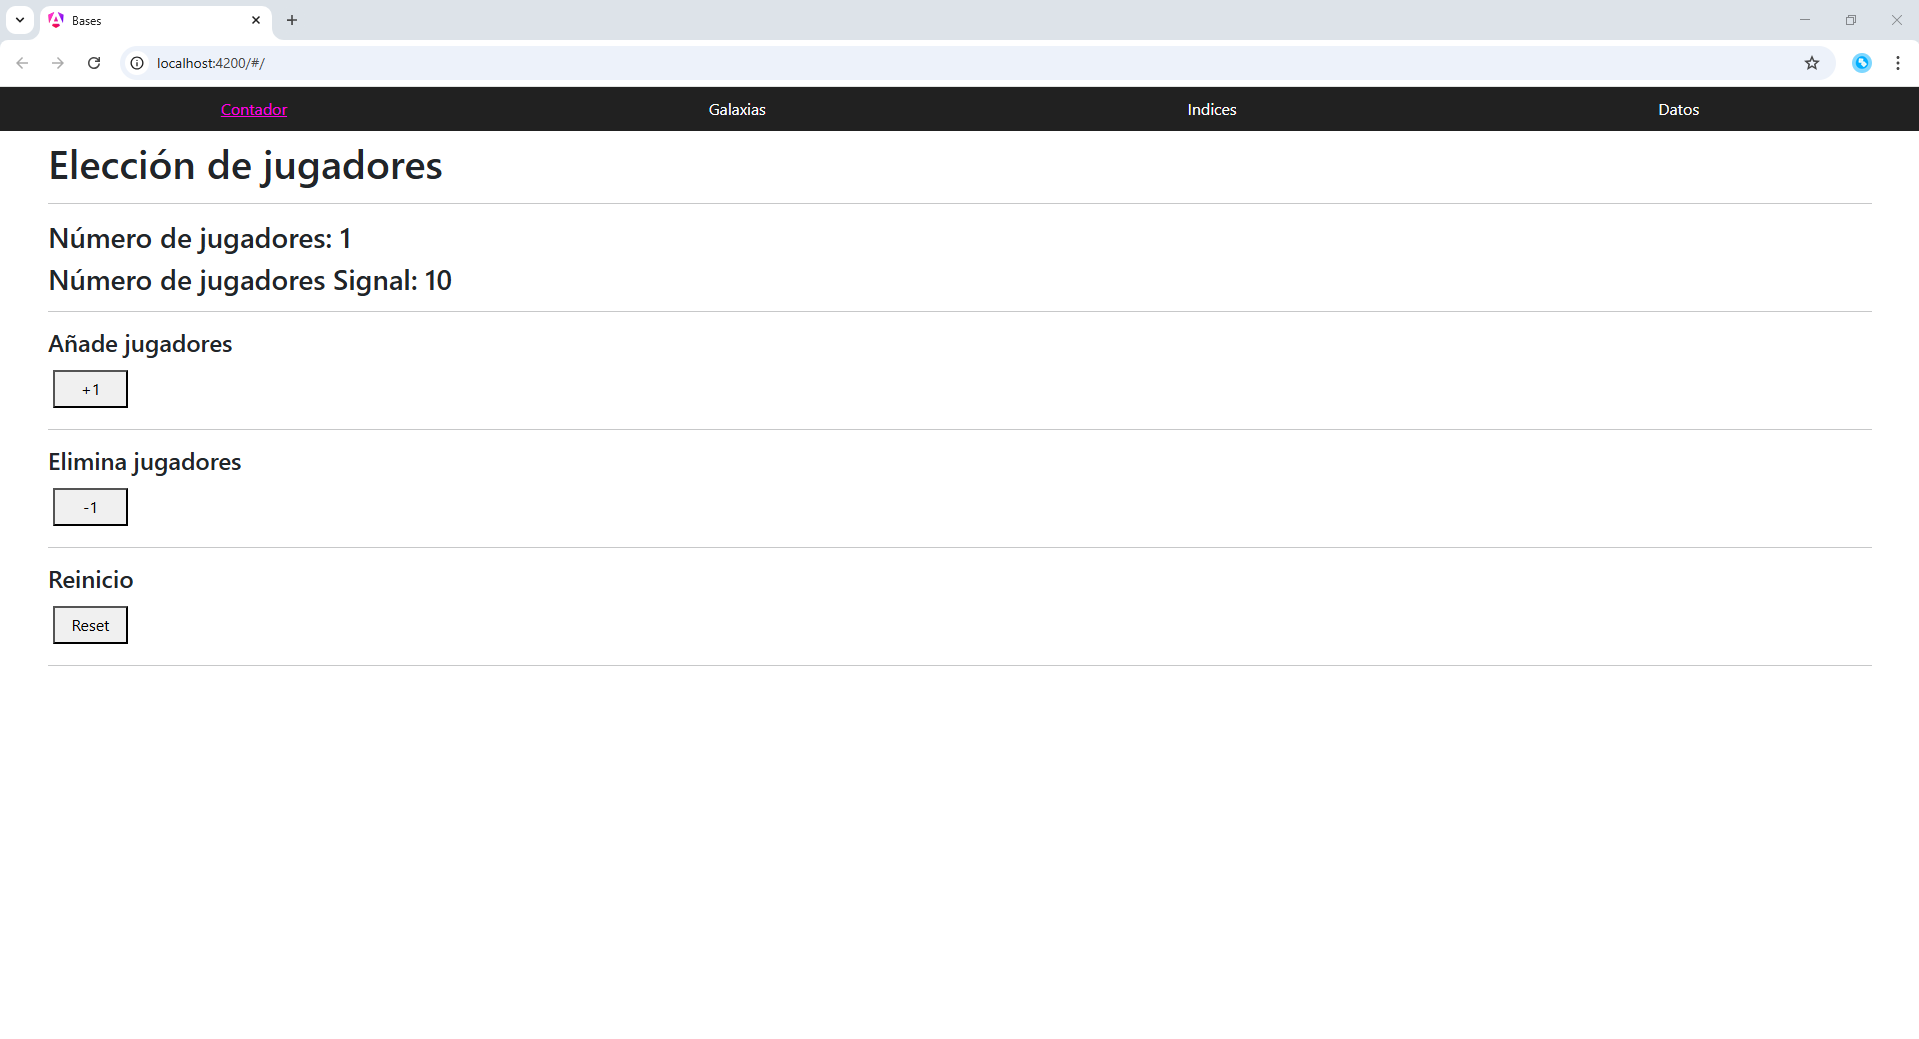
\includegraphics[width=0.8\linewidth]{figuras/pag1.png}
    \caption[Formulario web: Página 1]{En este se pueden agregar y disminuir\textit{jugadores} del entorno.}
    \label{pag1}
\end{figure}
\begin{figure}[H]
     \centering
    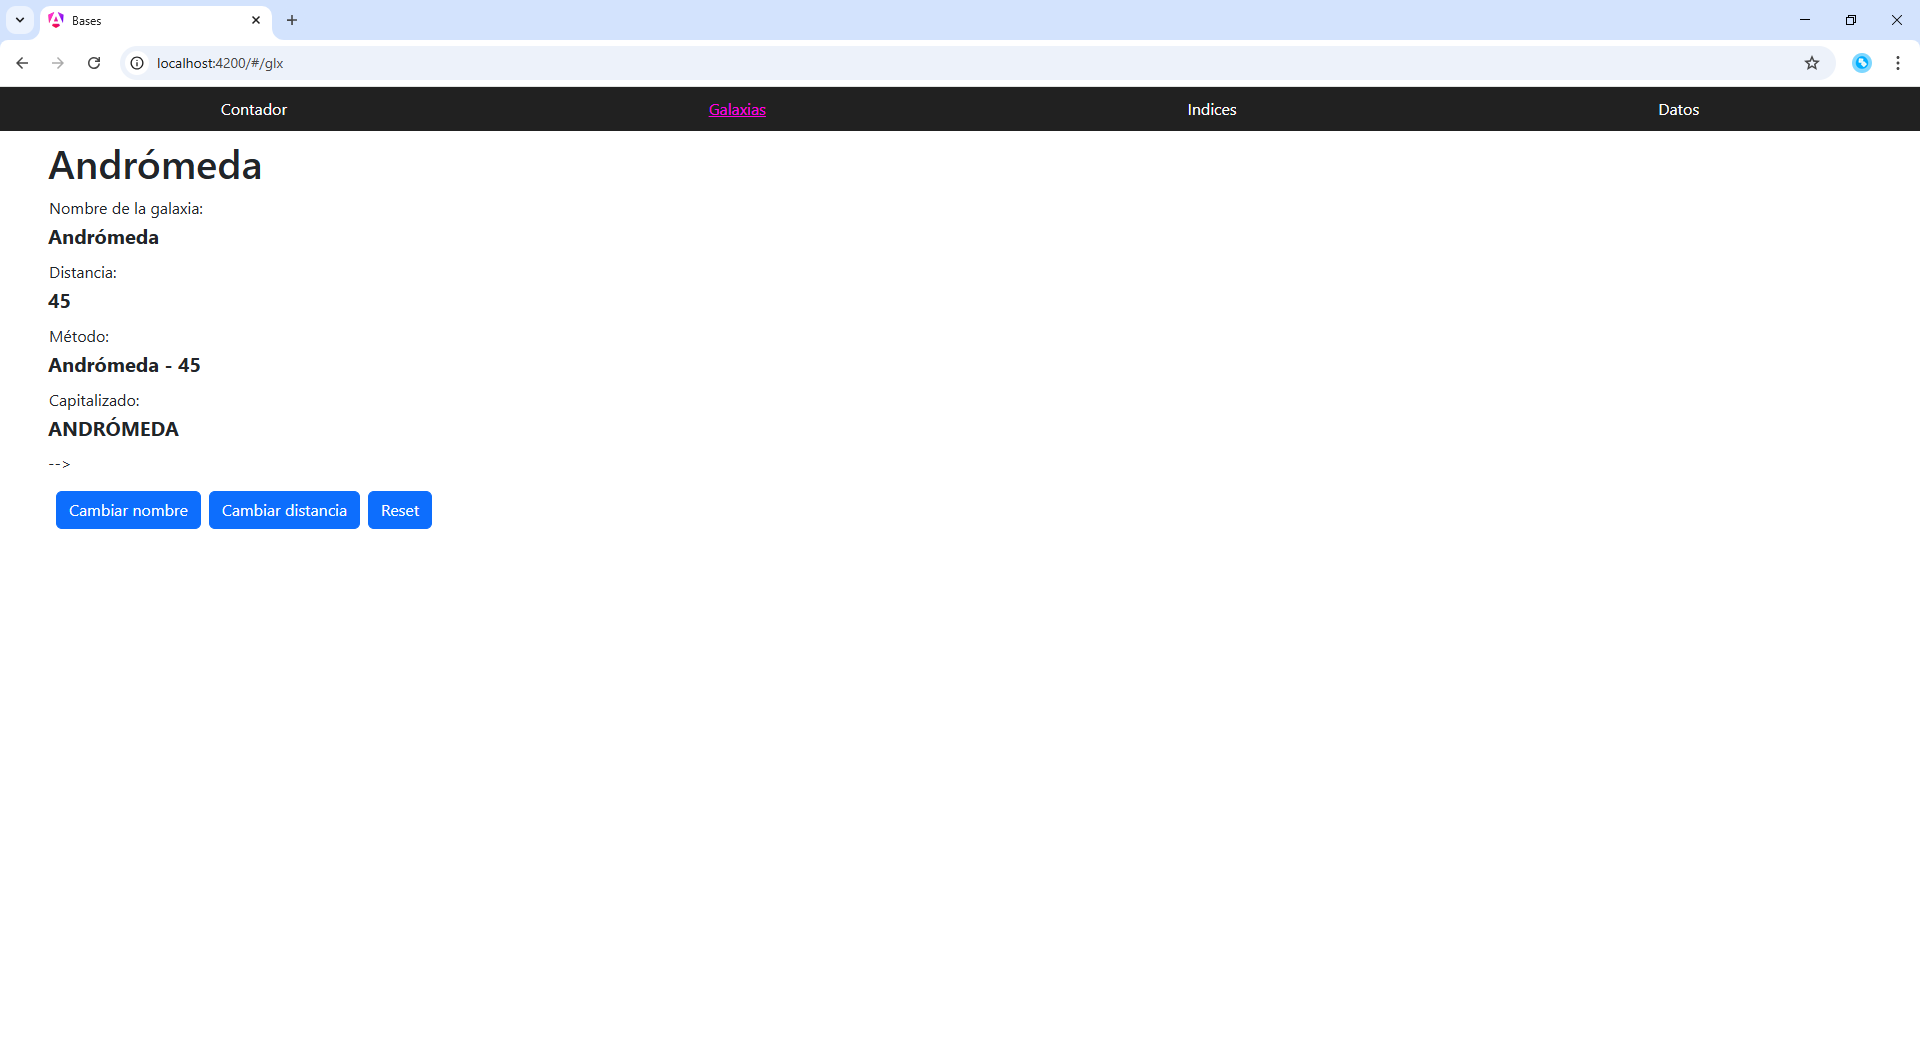
\includegraphics[width=0.8\linewidth]{figuras/pag2.png}
    \caption[Formulario web: Página 2]{Formulario que permite variar los datos de una galaxia restaurarlos por los iniciales.}
    \label{pag2}
\end{figure}
\begin{figure}[H]
\centering
    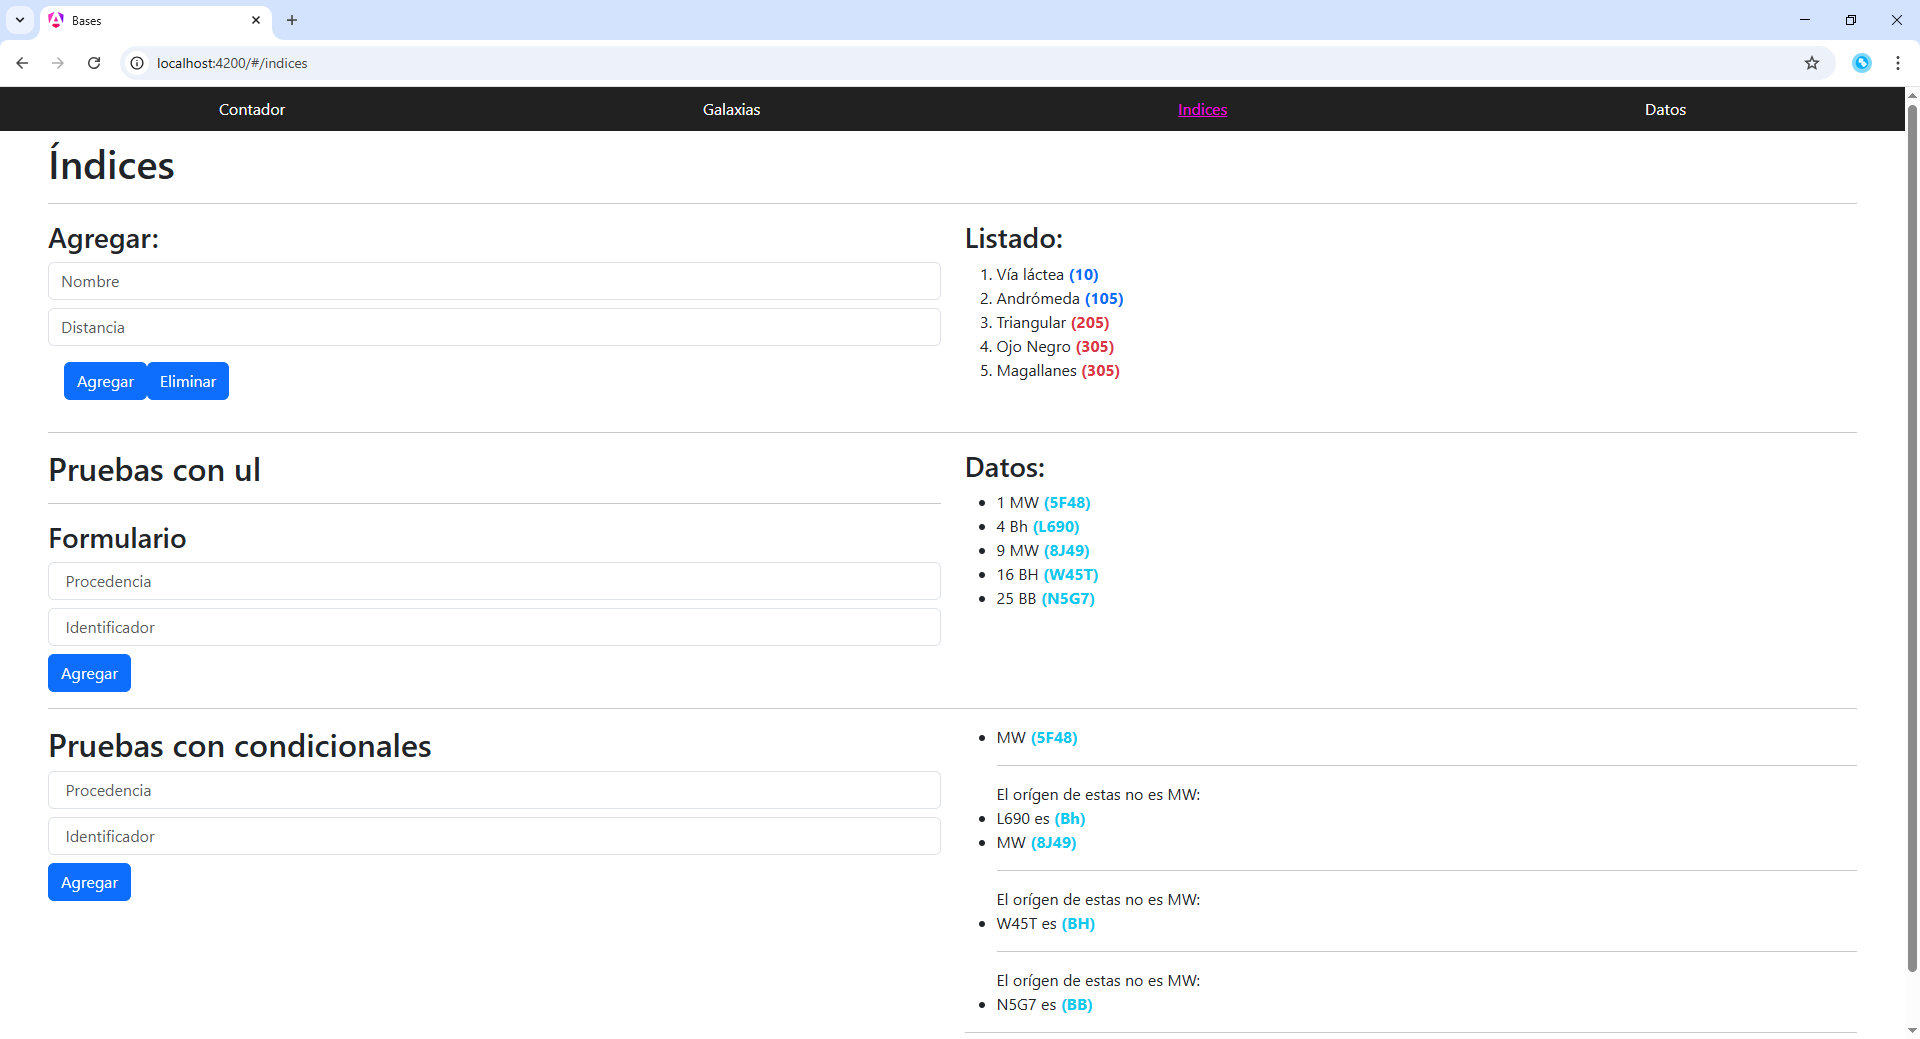
\includegraphics[width=0.8\linewidth]{figuras/pag3.png}
    \caption[Formulario web: Página 3]{En este entorno se permite agregar elementos a la lista de manera general o condicionada.}
    \label{pag3}
\end{figure}
\begin{figure}[H]
    \centering
    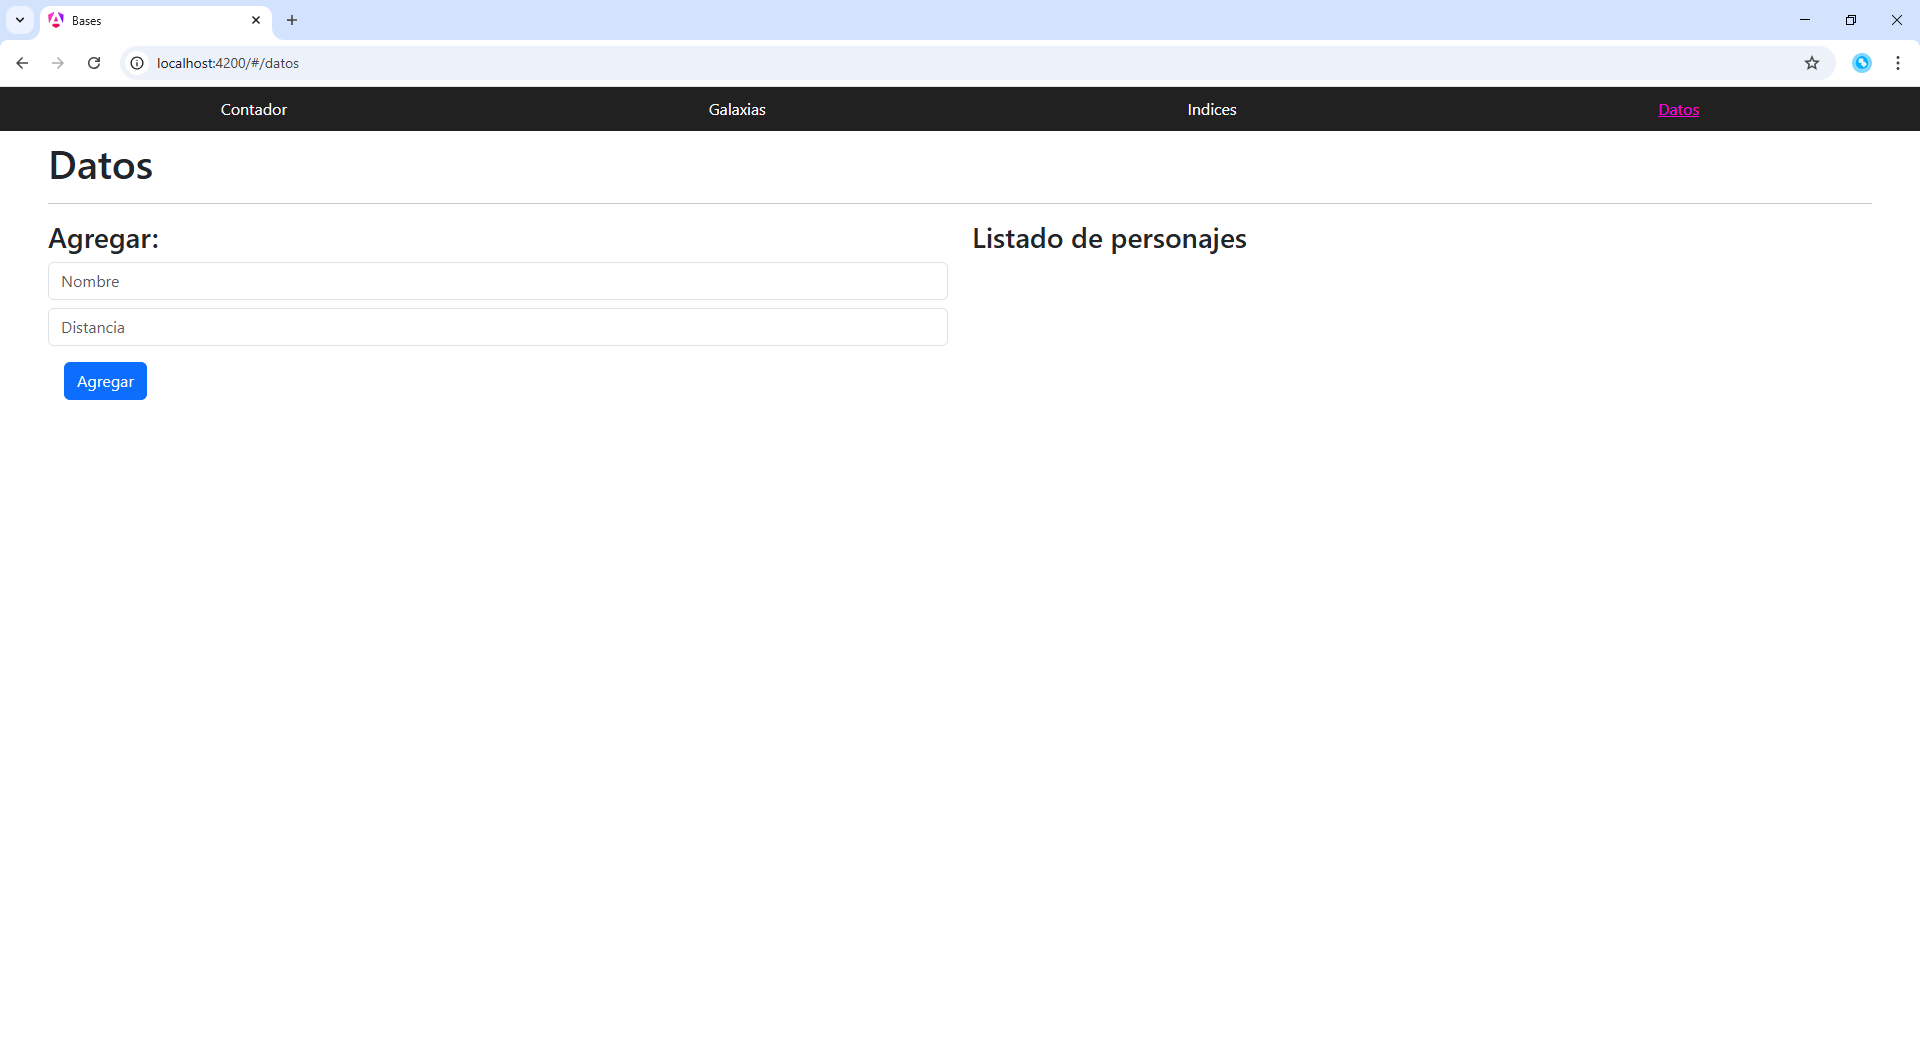
\includegraphics[width=0.8\linewidth]{figuras/pag4.png}
    \caption[Formulario web: Página 4]{Formulario similar a la anterior pero en este caso permitía operar con los datos mostrándolos transformados.}
    \label{pag4}
\end{figure}

En las figuras\footnote{La primera de ellas se corresponde con una prueba en la que se analizaba el comportamiento de distintas formas de definir variables en Angular y no tiene relación con las siguientes.} se muestran capturas de la primera página desarrollada, en la que se tenían diversos formularios, con sus \textit{URLs} específicas. Los datos, inventados naturalmente, hacían referencia al nombre de galaxias, distancia, origen e identificador. La funcionalidad de la página era la creación de formularios cuyos datos se agregaran a listas de manera general, condicionada (en este caso particular por el origen o la distancia). Además, se añadió la posibilidad de exponer los datos, cambiarlos o restaurarlos.

En segundo lugar, se procedió a la creación de una aplicación más elaborada, que tuviera un menú interactivo como capa principal y que registrara en él ciertos datos como el usuario o una foto de perfil.

El navegador se comportaba de manera reactiva, adaptándose al tamaño de la pantalla, tal y como se muestra en la \Cref{fotomenu}. A la izquierda de las imágenes puede apreciarse el menú lateral, en el que aparecen los ítems (en este caso, dos) que permiten acceder al resto de modalidades de la página.

\begin{figure}[H]
\centering
\begin{subfigure}[b]{0.55\textwidth}
\centering

\includegraphics[width=\textwidth]{figuras/foto1.png}
\caption[Navegador web en pantalla completa]{Imagen de navegador en pantalla completa.}
\label{foto1}
\end{subfigure}
\hfill
\begin{subfigure}[b]{0.55\textwidth}
\centering
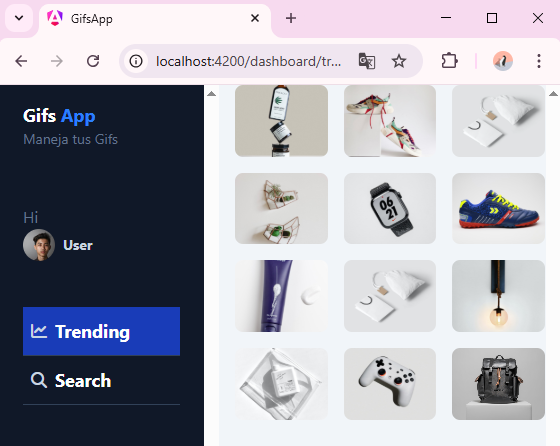
\includegraphics[width=\textwidth]{figuras/foto2.png}
\caption[Navegador web en pantalla reducida]{Imagen de navegador en pantalla reducida.}
\label{foto2}
\end{subfigure}
\caption{Segunda aplicación web con menú interactivo.}
\label{fotomenu}
\end{figure}

El repositorio de \textit{gifs} incorporado en la aplicación se organizaba mediante una pestaña denominada \textit{trending}, que permitía ordenarlos. En este caso, como es evidente, no se podía disponer de un registro de las consultas de los usuarios, por lo que las entradas se organizaban de manera alfabética.
%
%
\subsection{GCP}
%
%
Este entorno proporciona la infraestructura en la nube necesaria para desplegar aplicaciones, almacenar datos y ejecutar servicios de manera flexible y segura. La empresa Evenbytes es, como ya se ha mencionado, \textit{partner} de Google, por lo que brinda la posibilidad de trabajar con la mayor parte de funcionalidades de esta plataforma. Trabajar en la nube facilita el acceso compartido, la escalabilidad de los recursos y la automatización de procesos, lo que resulta especialmente valioso en proyectos donde intervienen varios miembros del equipo o que requieren alta disponibilidad.

En mi caso particular, implementé una \textit{Cloud Function} encargada de realizar el proceso de extracción de información de una página web (llamado \textit{web scraping}) y la generación de un fichero con los resultados. La \textit{Cloud Function} permite ejecutar fragmentos de código en respuesta a eventos o invocaciones programadas, sin necesidad accionar explícitamente el programa. Desde Python realicé el código para conectarse a la página de Wikipedia sobre cocientes intelectuales por país, extraer las tablas relevantes y convertir los datos en un archivo CSV. El código de la función se desplegó en GCP mediante las herramientas de línea de comandos y quedó configurado para ejecutarse de forma automática a intervalos regulares.

Para esta última tarea hice uso de Cloud Scheduler, un servicio que permite programar tareas basadas en cron. La configuración del Scheduler se gestionó a través de Terraform. Gracias a esta combinación, cada ejecución de la función generaba automáticamente un nuevo bucket \footnote{
Los buckets son contenedores que permiten almacenar objetos de manera segura y escalable. En este proyecto, cada bucket contenía los resultados de la extracción en formato CSV, de forma que quedaba un histórico de ejecuciones accesible a través de la consola de GCP o mediante las APIs correspondientes.} de almacenamiento en Cloud Storage, en el que se guardaba el fichero CSV con los datos actualizados.

A continuación se muestran fragmentos de código de la programación del \textit{web scraping}, la planificación en Terraform y el resultado del CSV. 
\begin{figure}[H]
\centering
\begin{subfigure}[b]{0.48\textwidth}
\centering
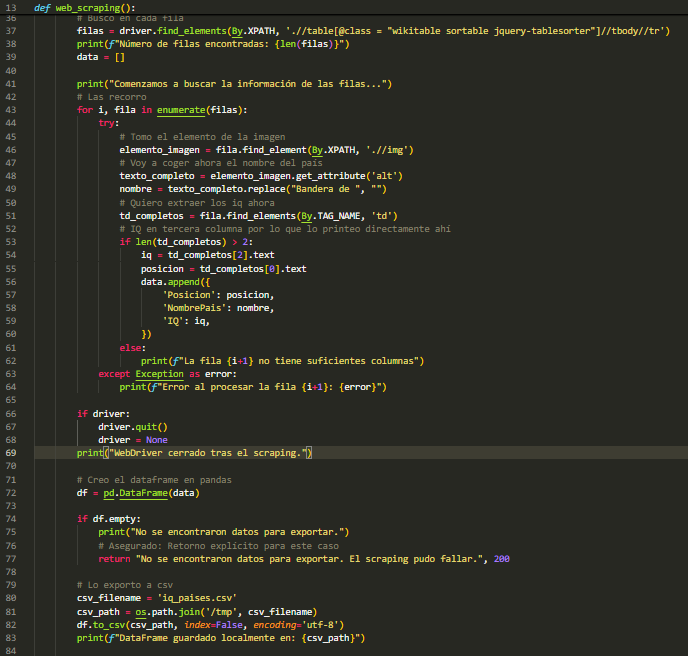
\includegraphics[width=\textwidth]{figuras/captura_webscraping.png}
\caption[Fragmento del código de web scrapping]{Fragmento del código de \textit{web scraping} en Python \cite{AlcamsodMemoria}.}
\label{webscraping}
\end{subfigure}
\hfill
\begin{subfigure}[b]{0.49\textwidth}
\centering
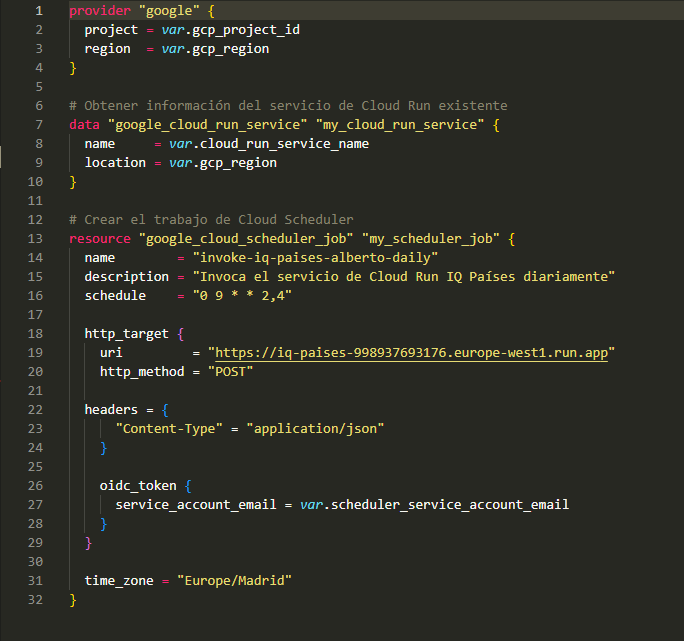
\includegraphics[width=\textwidth]{figuras/captura_terraform.png}
\caption[Fragmento del código del scheduler]{Ejemplo de configuración de Terraform para el \textit{scheduler} \cite{AlcamsodMemoria}.}
\label{terraform}
\end{subfigure}
\caption{Fragmentos código entorno GPC.}
\label{TerraformWebScraping}
\end{figure}
A modo de breve explicación de los códigos mostrados, para el caso del \textit{web scraping} la idea principal es generar un navegador virtual al que se le manda a la página de la que queremos extraer los datos. De manera previa, se investiga el código HTML para saber la estructura de la página, de modo que creamos un bucle que busque los elementos que queremos y extraiga la información de ellos, es decir, si tenemos una estructura en la que todos los objetos tienen una propiedad llamada \textit{nombre}, hacemos que nuestro código acceda a él para extraer todos los nombres de la página y guardarlos en un fichero.

Por otro lado, el scheduler es más sencillo, le introducimos los datos del proyecto, función a llamar... y definimos las órdenes bajo las que se ejecuta. En el código aparece en la línea 16 el fragmento \textit{0 9 * * 2,4} que significa que se ejecute a las \textit{9:00}, \textit{cualquier día} (numérico), \textit{cualquier mes}, los \textit{martes} y \textit{jueves}.
%
%
\subsection{GitHub}
%
%
En último lugar estuvo el aprendizaje de GitHub, que actúa como sistema de control de versiones, permitiendo gestionar el historial de cambios en el código, coordinar el trabajo y asegurar que todas las contribuciones queden registradas de forma ordenada. Su uso es fundamental en un entorno profesional, ya que permite mantener la trazabilidad de los desarrollos, revisar modificaciones y garantizar la integridad de los proyectos a medida que evolucionan. Su estructura es muy sencilla y puede entenderse rápidamente pensando en grafos. Se crea una rama principal del proyecto y de ellas, cuando se quiere trabajar en una parte específica del mismo, salen hijas. De esta manera los cambios realizados se hacen fuera del proyecto principal, permitiendo guardar los cambios, avanzar únicamente en esa línea o abrir nuevas. Cuando una parte se da por revisada y acabada se unen ramas a la principal (padre), de manera que se va completando el trabajo. Los comandos básicos de Git son \textit{commit}, que guarda los cambios realizados en el repositorio local; \textit{pull}, que actualiza la copia local con las modificaciones del repositorio remoto; \textit{push}, que sube los cambios locales al repositorio compartido; y \textit{merge}, que combina diferentes ramas en una sola versión final.
\begin{figure}[H]
    \centering
    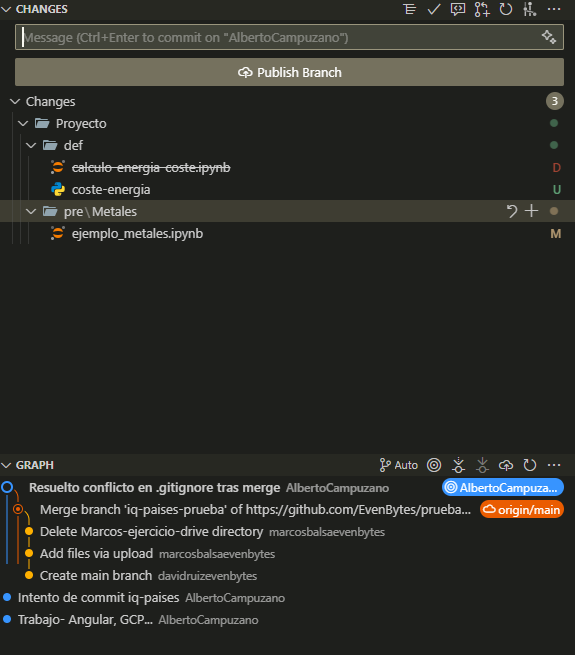
\includegraphics[width=0.42\linewidth]{figuras/captura_github.png}
    \caption[Interfaz de GitHub en Visual Code]{Imagen GitHub}
    \label{GitHub}
\end{figure}
%
%
